\section{Nhận diện biển báo giao thông}
Hệ thống nhận diện thường liên quan đến hai nhiệm vụ chính: phát hiện, bao gồm:
\begin{enumerate}
    \item \textbf{Detection: }xác định vị trí và kích thước của đối tượng trong ảnh đầu vào
    \item \textbf{Classification: } gán các đối tượng đã phát hiện vào các lớp con cụ thể
\end{enumerate}
Nhóm đã quyết định tích hợp một mô hình học máy vào hệ thống để cung cấp hỗ trợ trong quá trình nhận diện và phân loại. Để huấn luyện mô hình này, ta cần sử dụng dữ liệu có nhãn. Thay vì phải tự thu thập và gán nhãn, nhóm đã chọn và tận dụng hai bộ dữ liệu có sẵn là GTSDB (German Traffic Sign Detection Benchmark) và GTSRB (German Traffic Sign Recognition Benchmark).


\subsection{Giai đoạn 1: Xác định vị trí biển báo}
\subsubsection{Một số khái niệm}

\subsubsection{Giới thiệu YOLO}
YOLO chia một bức ảnh đầu vào thành một ô lưới có kích thước S×S. Giá trị S được chọn bằng 7 trong paper. Nếu tâm của một vật thể rơi vào một ô nào thì ô đó sẽ chịu trách nhiệm cho việc tìm kiếm vật thể đó.

\begin{figure}[htp]
  \centering
  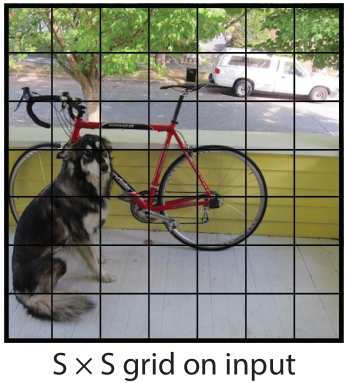
\includegraphics[width=0.4\textwidth]{images/2a-sign/grid1.png}
  \caption{Lưới 7x7}
\end{figure}

\noindent Hình trên là một ví dụ về một bức ảnh đầu vào được chia thành một ô lưới có kích thước S×S. Trong YOLO, giá trị S được chọn bằng 7. 
Mỗi grid cell sẽ dự đoán B bounding boxes và confidence score cho mỗi box đó. Ta sẽ xét kỹ hơn hai khái niệm này ngay dưới đây.\\

\noindent Confidence score sẽ phản ánh hai thông số:
\begin{itemize}
    \item Mức độ tự tin của mô hình trong việc dự đoán box đó chứa vật thể.
    \item Độ chính xác của predicted box là bao nhiêu (tức box đó khớp với ground-truth box đến mức nào).
\end{itemize}
Từ hai ý trên, ta định nghĩa confidence score một cách chặt chẽ hơn như sau: $Pr(Object)$ x $IOU^{truth}_{pred}$.\\
Từ công thức trên, ta có thể rút ra một vài nhận xét như sau:
\begin{itemize}
    \item Nếu không có vật thể nào tồn tại trong cell đó thì  p(Object) = 0 $\Rightarrow$ confidence score = 0.
    \item Ngược lại, nếu cell đó chứa vật thể $\Rightarrow$ p(Object) = 1, , vì thế ta kỳ vọng confidence score = IOU giữa predicted box và ground truth box.
\end{itemize}
Mỗi bounding box thể hiện 5 giá trị x, y, w, h, confidence:
\begin{itemize}
    \item (x, y) là tọa độ tâm (offset) của bounding box so với với vị trí của của grid cell, vì thế nên giá trị của x, y sẽ rơi vào đoạn [0,1].
    \item w, h là width, height của bounding boxes, được chuẩn hóa theo width và height của bức ảnh gốc, vì thế giá trị của chúng sẽ rơi vào đoạn [0,1].
    \item Confidence biểu diễn giá trị IOU giữa predicted box và ground truth box.
    \begin{figure}[htbp]
        \centering
        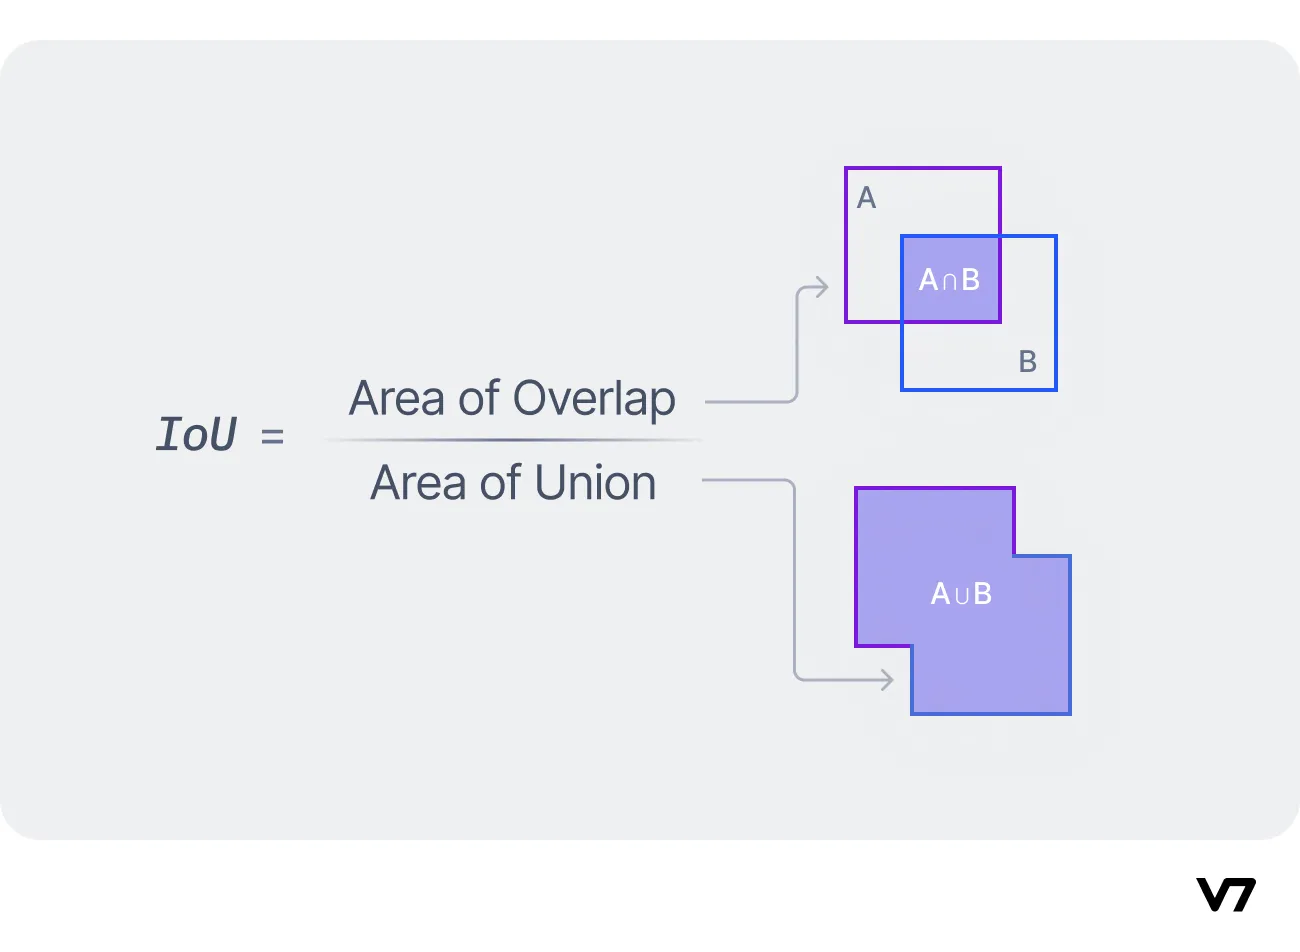
\includegraphics[width=0.6\textwidth]{images/2a-sign/IOU.png}
        \caption{Intersection over Union}
    \end{figure}
\end{itemize}
Mỗi grid cell cũng sẽ dự đoán C xác suất có điều kiện của các class: $p(Class_{i}|Object)$ (Các xác suất này được lấy điều kiện trên grid cell chứa đối tượng).

\noindent Tại thời điểm test, ta nhân xác suất có điều kiện của mỗi class với dự đoán confidence của từng box như sau: 
\begin{center}
    $p(Class_{i}|Object)$ x $p(Object$ x $IOU^{truth}_{pred}$ = $p(Class_{i})$ x $IOU^{truth}_{pred}$
\end{center}
Công thức trên cho ta confidence scores của từng class cho mỗi box. Công thức này cho ta biết:
\begin{itemize}
    \item Xác suất của $class_i$ xuất hiện trong box đó
    \item Độ khớp của của predicted box so với vật thể.
\end{itemize}
Như vậy, có thể tóm gọn lại quy trình hoạt động của YOLO như sau:
\begin{figure}[htbp]
        \centering
        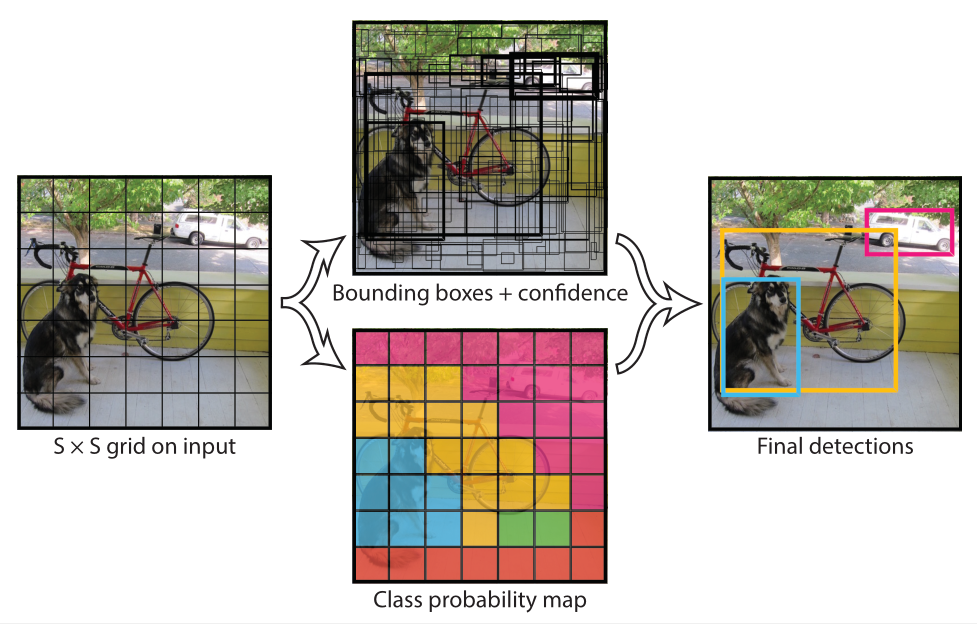
\includegraphics[width=0.6\textwidth]{images/2a-sign/grid2.png}
        \caption{Quy trình của YOLO}
\end{figure}
Trong phạm vi của đề tài này, quyết định của nhóm là sử dụng mô hình YOLOv3 để thực hiện nhiệm vụ nhận diện và định vị đối tượng. Để hiểu rõ hơn về lựa chọn này, nhóm sẽ giới thiệu không chỉ về YOLOv3 mà còn về các phiên bản trước đó bao gồm YOLOv1 và YOLOv2. Điều này giúp ta có cái nhìn tổng quan về sự tiến triển và cải tiến của mô hình YOLO theo thời gian, cũng như lý do mà YOLOv3 được chọn làm nền tảng cho nghiên cứu và thực nghiệm của nhóm.

\subsubsection{YOLOv1}
\myparagraph{Kiến trúc}
Kiến trúc mạng YOLOv1 được lấy ý tưởng từ mô hình GoogLeNet cho phân loại ảnh. Nó gồm có 24 Convolutional Layers dùng để trích xuất các features từ bức ảnh, theo sau bởi 2 Fully Connected Layers để dự đoán output probabilities và coordinates. Thay vì sử dụng inception modules trong GoogLeNet, YOLO chỉ sử dụng reduction layers có kích thước 1x1 theo sau bởi Convolutional Layers có kích thước 3x3 
\begin{figure}[htbp]
        \centering
        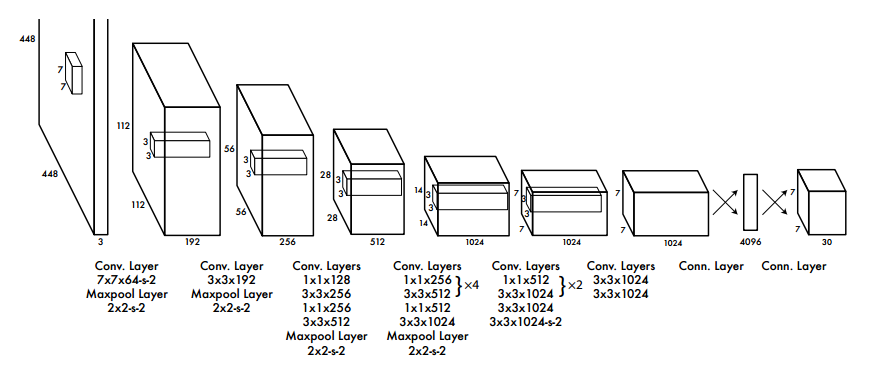
\includegraphics[width=0.8\textwidth]{images/2a-sign/yolo1_arch.png}
        \caption{Kiến trúc YOLOv1}
\end{figure}

\myparagraph{Hàm mất mát}
\begin{figure}[htbp]
        \centering
        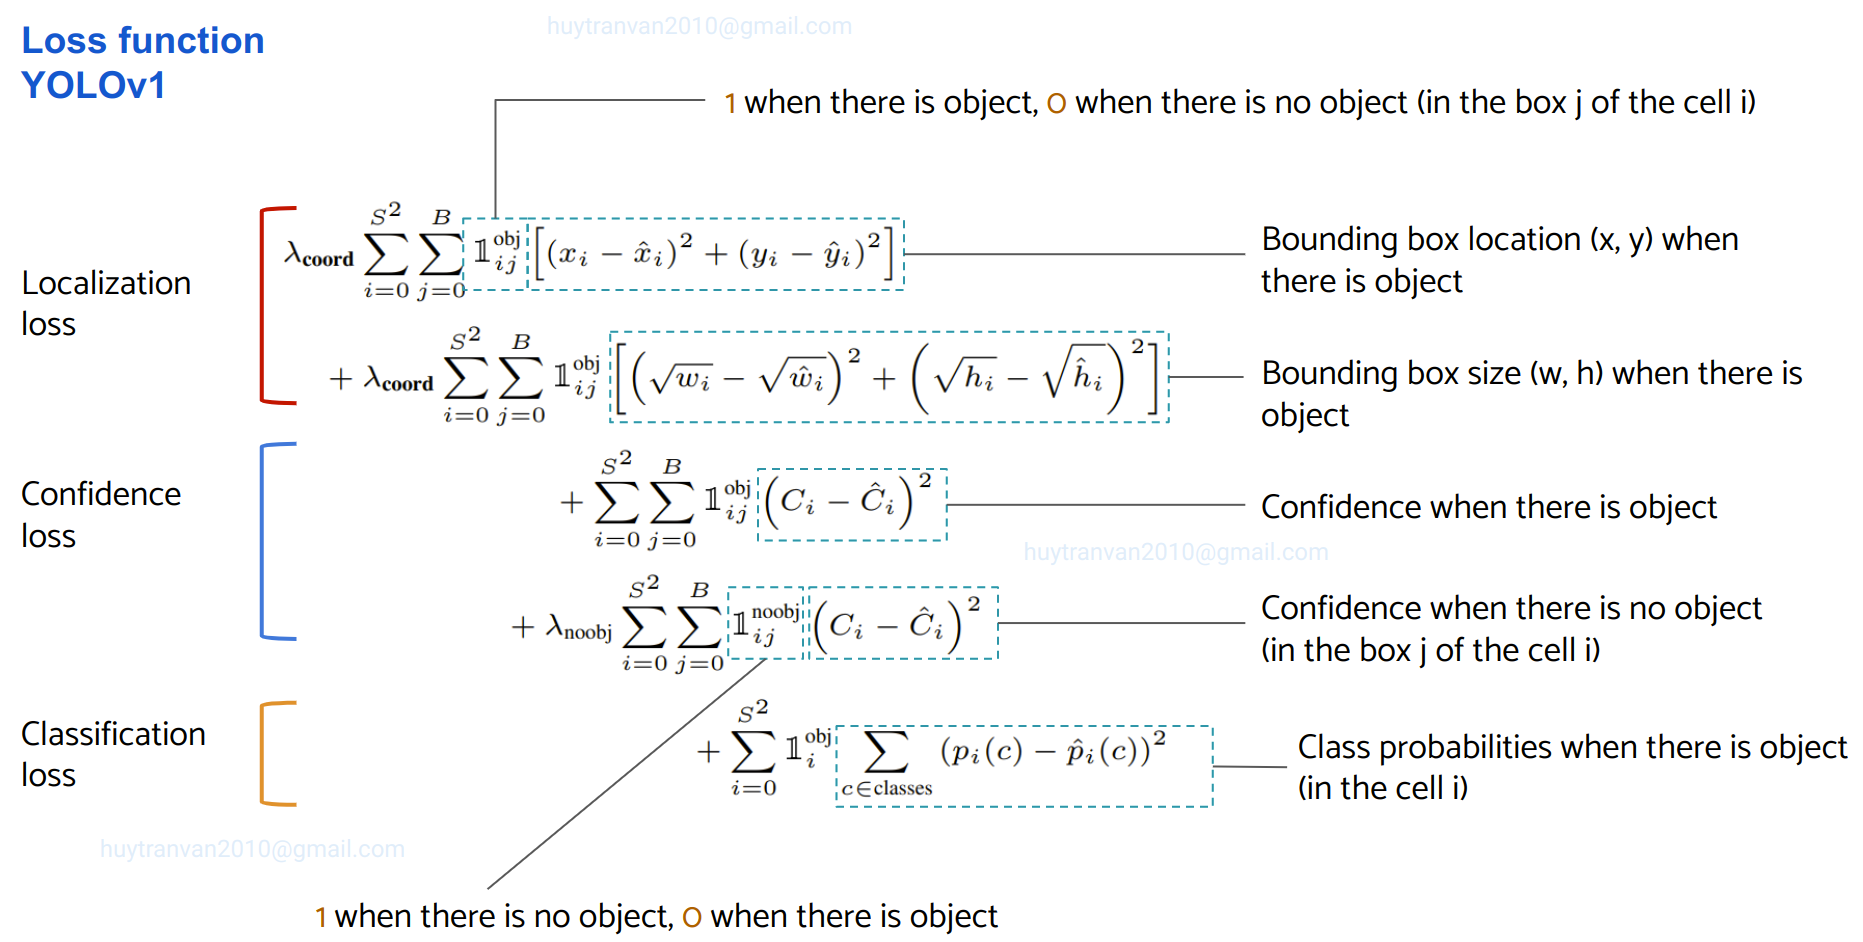
\includegraphics[width=0.8\textwidth]{images/2a-sign/YOLO_loss.png}
        \caption{Hàm mất mát tổng quát}
\end{figure}
\begin{itemize}
    \item \textbf{Localization loss}
    \begin{equation*}
\mathcal{L}_{loc} = \lambda_{coord} \sum_{i=0}^{S^2} \sum_{j=0}^B \mathds{1}_{ij}^{obj} [(x_i - \hat{x}_i)^2 + (y_i - \hat{y}_i)^2 ] +\lambda_{coord} \sum_{i=0}^{S^2} \sum_{j=0}^B \mathds{1}_{ij}^{obj} [(\sqrt{w_i} - \sqrt{\hat{w}_i})^2 + (\sqrt{h_i} - \sqrt{\hat{h}_i})^2]
    \end{equation*}
$\mathds{1}_{i}^{obj}$ = 1 thể hiện trong cell i có object xuất hiện (ngược lại thì bằng 0).\\
$\mathds{1}_{i}^{obj} = 1$ nếu box j của grid cell i có chứa object, ngược lại bằng 0. Ở đây grid cell i phải chứa object trước đã, chứa object rồi thì mới khớp được với prediected box.\\

Khi huấn luyện chúng ta đã biết grounth-truth box thuộc cell nào. Khi dự đoán đưa ra nhiều predicted boxes cho mỗi grid cell. Chúng ta chỉ muốn duy nhất một predicted box chịu trách nhiệm cho object của grid cell. Do đó box thứ j được coi chứa object trong grid cell i là predicted box có IoU cao nhất trong 2 boxes thuộc grid cell đó. Trong hoàn cảnh này tất nhiên đang đề cập đến grid cell i
 có object.
\begin{figure}[htbp]
    \centering
    \subfigure[htp]{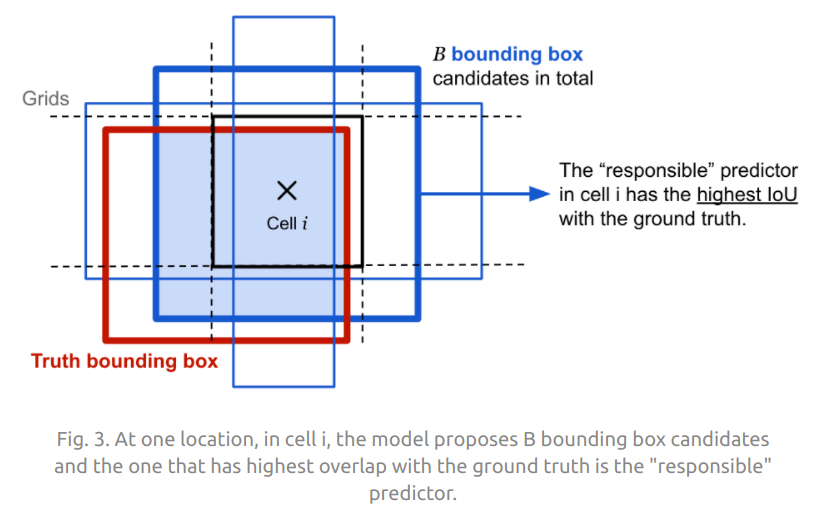
\includegraphics[width=0.4\textwidth]{images/2a-sign/L-loss1.png}}
    \subfigure[htp]{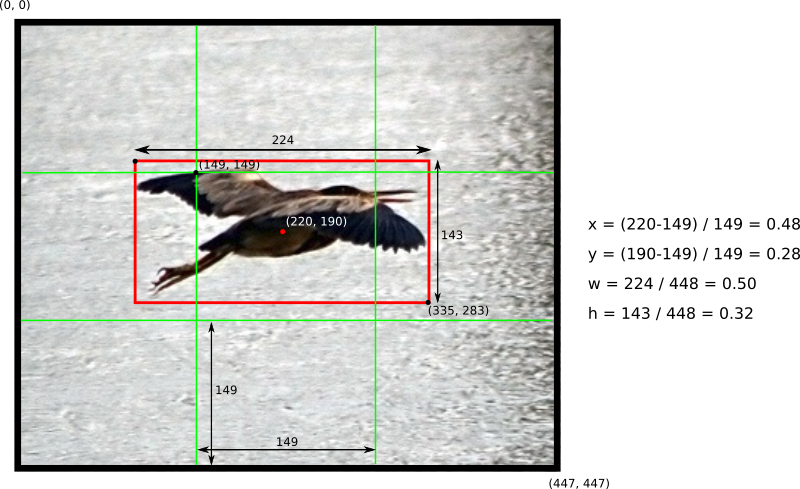
\includegraphics[width=0.4\textwidth]{images/2a-sign/L-loss2.png}}
\end{figure}

Trong loss function $\mathcal{L}_{loc}$ nhận thấy width và height dùng square root (căn bậc 2). Điều này để tính đến việc chênh lệch giữa hai box lớn ít bị ảnh hưởng hơn so với chênh lệch giữa hai box nhỏ. Cùng lấy ví dụ để hiểu rõ hơn. Ví dụ chúng ta lấy $\omega_1 = 0.55$, $\hat{\omega}_1 = 0.5$, $\omega_2 = 0.5$, $\hat{\omega}_2 = 0.45$, nhận thấy $\omega_1 - \hat{\omega}_1 = 0.5 = \omega_2 -\hat{\omega}_2$, tuy nhiên bounding boxes nhỏ hơn $\omega_2 = 0.5$, $\hat{\omega}_2 = 0.45$ bị lệch nhiều hơn so với bounding boxes lớn $\omega_1 = 0.55$, $\hat{\omega}_1 = 0.5$. Vì vậy, lấy căn bậc 2 của giá trị này sẽ làm giảm độ ảnh hưởng của Bounding Box lớn khi có lệch nhỏ. 
    \item \textbf{Confidence loss (hay object loss)}
    \begin{equation*}
        \mathcal{L}_{obj} = {\sum_{i=0}^{S^2} \sum_{j=0}^B \mathds{1}_{ij}^{obj} (C_{ij} - \hat{C}_{ij})^2} +\lambda_{noobj}{\sum_{i=0}^{S^2} \sum_{j=0}^B \mathds{1}_{ij}^{noobj} (C_{ij} - \hat{C}_{ij})^2}
    \end{equation*}
Thành phần thứ nhất của object loss chính là phần loss cho trường hợp cell i có chứa objet, tức là $C_i = 1, C_{ij} = 1,\hat{C}_{ij} = Pr(object) . IOU_{pred}^{truth}$ là giá trị dự đoán cho bounding box j thuộc cell i.\\
Thành phần thứ nhất của object loss chính là phần loss cho trường hợp ngược lại, cell i không chứa objet, tức là $C_i = 0, C_{ij} = 0,\hat{C}_{ij} = Pr(object) . IOU_{pred}^{truth}$ là giá trị dự đoán cho bounding box j thuộc cell i.\\

$\mathds{1}_{ij}^{obj} = 1 (\mathds{1}_{ij}^{noobj} = 0)$ nếu box j của cell i có chứa vật thể, và $\mathds{1}_{ij}^{obj} = 0 (\mathds{1}_{ij}^{noobj} = 1)$ cho trường hợp ngược lại. Ở đây cứ grid cell và box của nó không match với nhau thì cho vào nhóm này, bao gồm cả những grid cell không chứa object và grid cell chứa object nhưng không khớp với box do có IoU nhỏ hơn box còn lại. Và những trường hợp không khớp như này chúng ta chỉ đi minimize objectness score, không quan tâm đến coordinates và class probabilities (vì vốn dĩ đã không chứa object).
\begin{figure}[htbp]
        \centering
        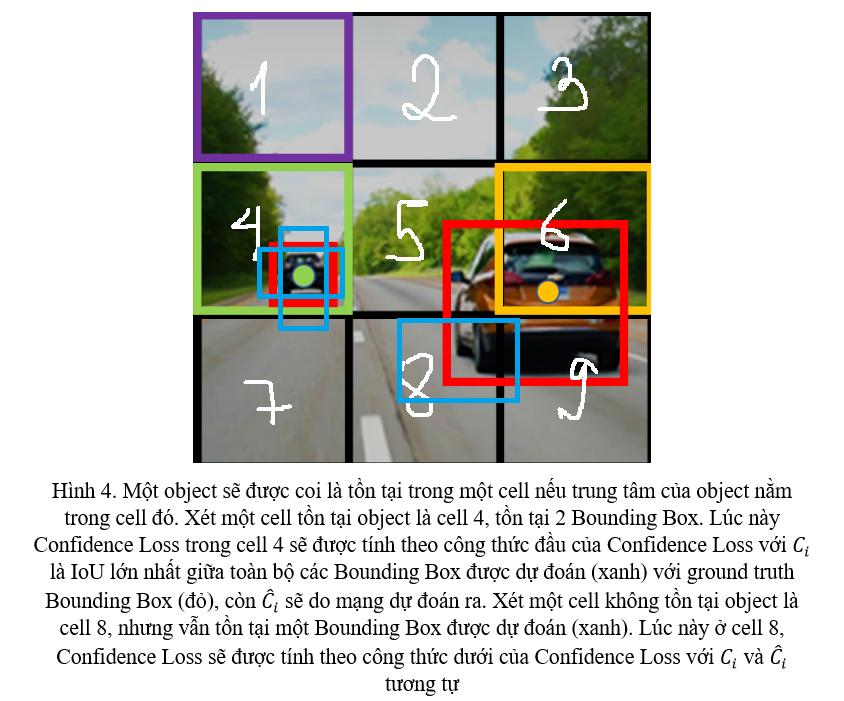
\includegraphics[width=0.5\textwidth]{images/2a-sign/L-loss3.png}
        \caption{Minh họa confidence loss}
\end{figure}

Ở đây, có một điều cần chú ý là trong ảnh đa số các grid cell không chứa object nên nếu để weights của localization loss và confidence loss cho vị trí không có object như nhau thì kết quả sẽ không tốt. Model lúc này có xu hướng tập trung dự đoán các box không chứa object để giảm loss nhiều nhất có thể. Do đó ở đây sẽ thiết lập weights khác nhau $\lambda_\text{noobj} =0.5, \lambda_\text{coord} = 5$ để tăng hiệu suất của model.
    \item \textbf{Classification loss}
\begin{equation*}
    \mathcal{L}_{cls}={\sum_{i=0}^{S^2} \mathds{1}_i^{obj}  \sum_{c \in classes} (p_i(c) - \hat{p}_i(c))^2}
\end{equation*}
trong đó $1^{obj}_{i}=1$ nếu grid cell thứ i chứa object.\\

$p_i(c)=Pr(class_i \mid object)$ được tính chung cho cả grid cell không phụ thuộc vào số bounding boxes của grid cell. Phần loss này chung cho grid cell có chứa object. Nếu class nào xuất hiện trong grid cell đó thì ta có $p(c) = 1$, các classes còn lại bằng 0.
\end{itemize}

\myparagraph{Non-Max Suppression}
Chú ý khi nhận diện có rất nhiều bounding boxes có thể phụ trách cho một vật thể. Để loại bỏ bớt các bounding boxes thừa chúng ta sẽ áp dụng Non-Max Supression. Tuy nhiên trước tiên chúng ta cần biến đổi ouput một chút. Ở bên trên chúng ta cũng đã đề cập:
\[
Pr(class_i | object) \cdot Pr(object) \cdot IOU_{pred}^{truth} = Pr(class_i) \cdot IOU_{pred}^{truth}
\]
Tương ứng với mỗi bounding box chúng ta sẽ có 20 giá trị $Pr(class_i) \cdot IOU_{pred}^{truth}$ thể hiện score của từng class trong bounding box có tính đến sự khớp với ground truth box. Tổng cộng chúng ta có $98 \times 20 = 1960$  các giá trị như này cho 98 bounding boxes do mỗi có $7 \times 7$ grid cell, mỗi cell có 2 boxes. Thực chất việc đưa về tensor $7 \times 7 \times 30 = 1470$ giúp chúng ta giảm số tham số trong mô hình thay vì phải dùng FC layer với 1960 units. Sau FC layer với 1470 units chúng ta reshape lại về tensor $7 \times 7 \times 30$  như hình bên dưới.
\begin{figure}[htbp]
        \centering
        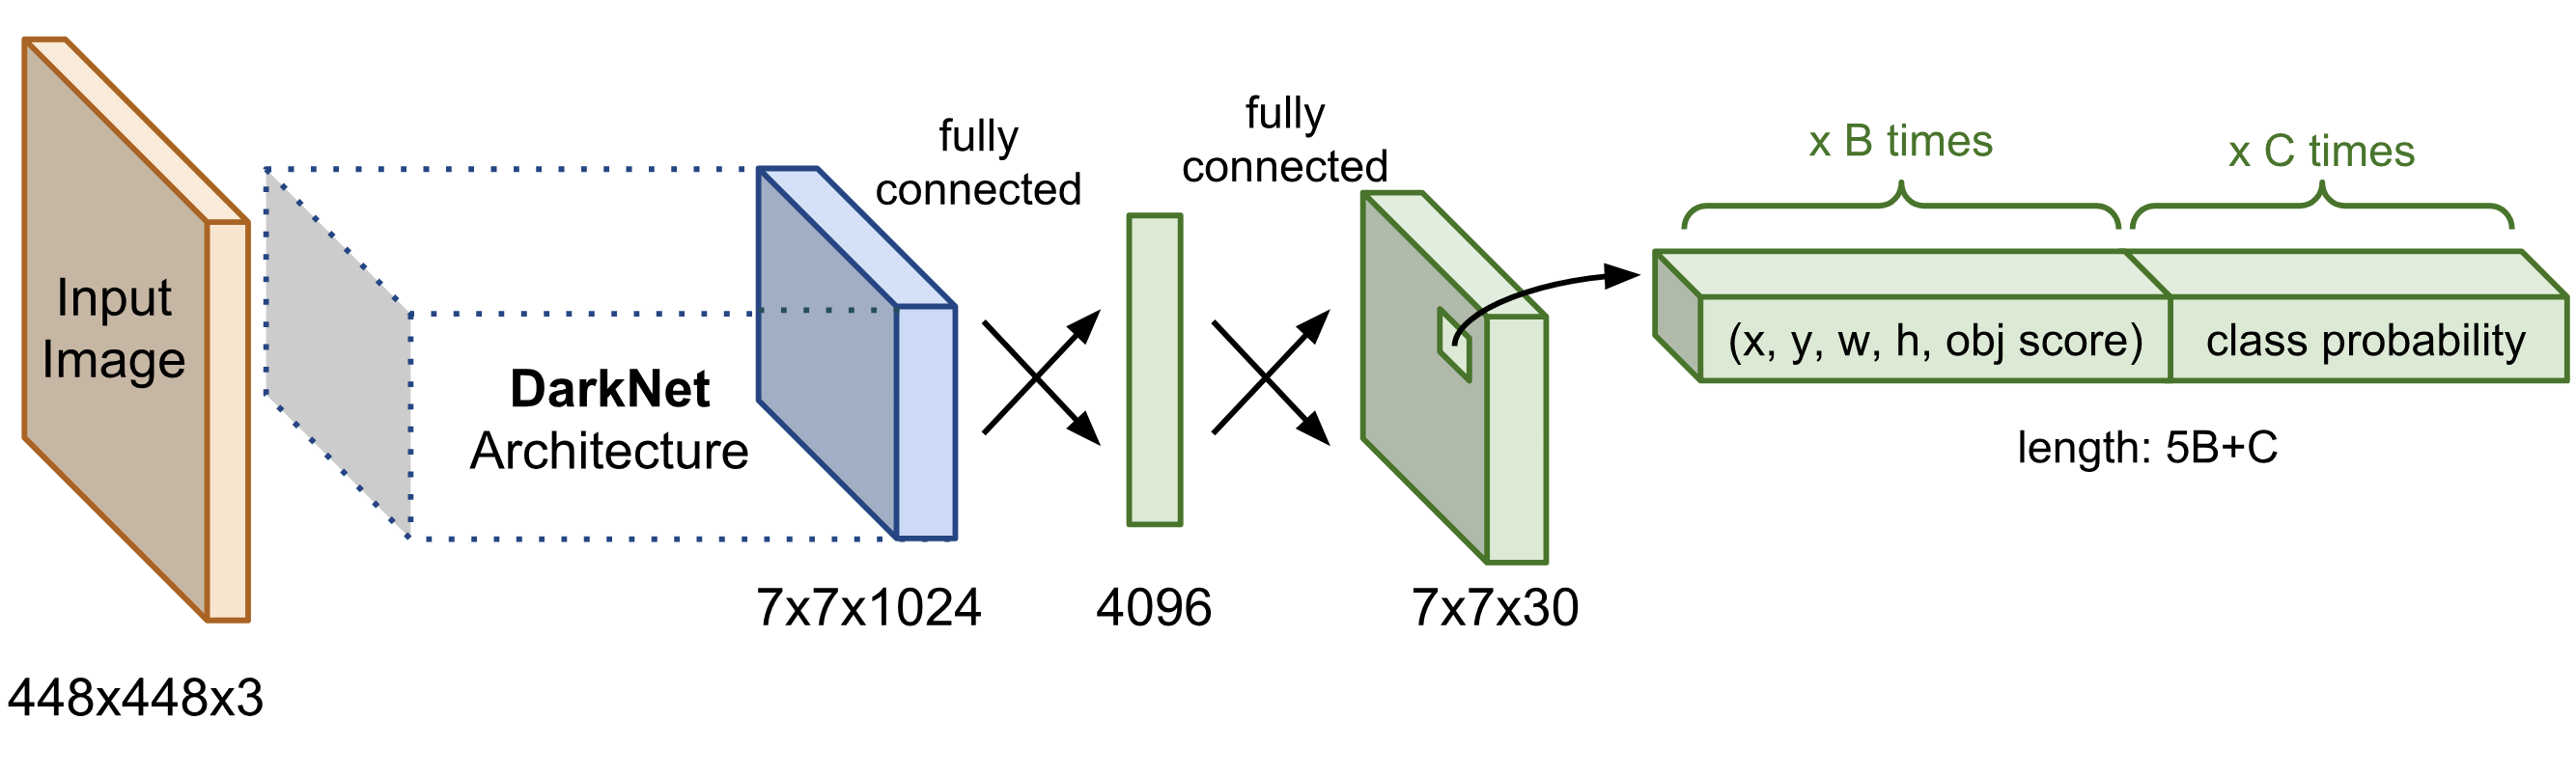
\includegraphics[width=0.6\textwidth]{images/2a-sign/1.png}
\end{figure}

\begin{figure}[htbp]
        \centering
        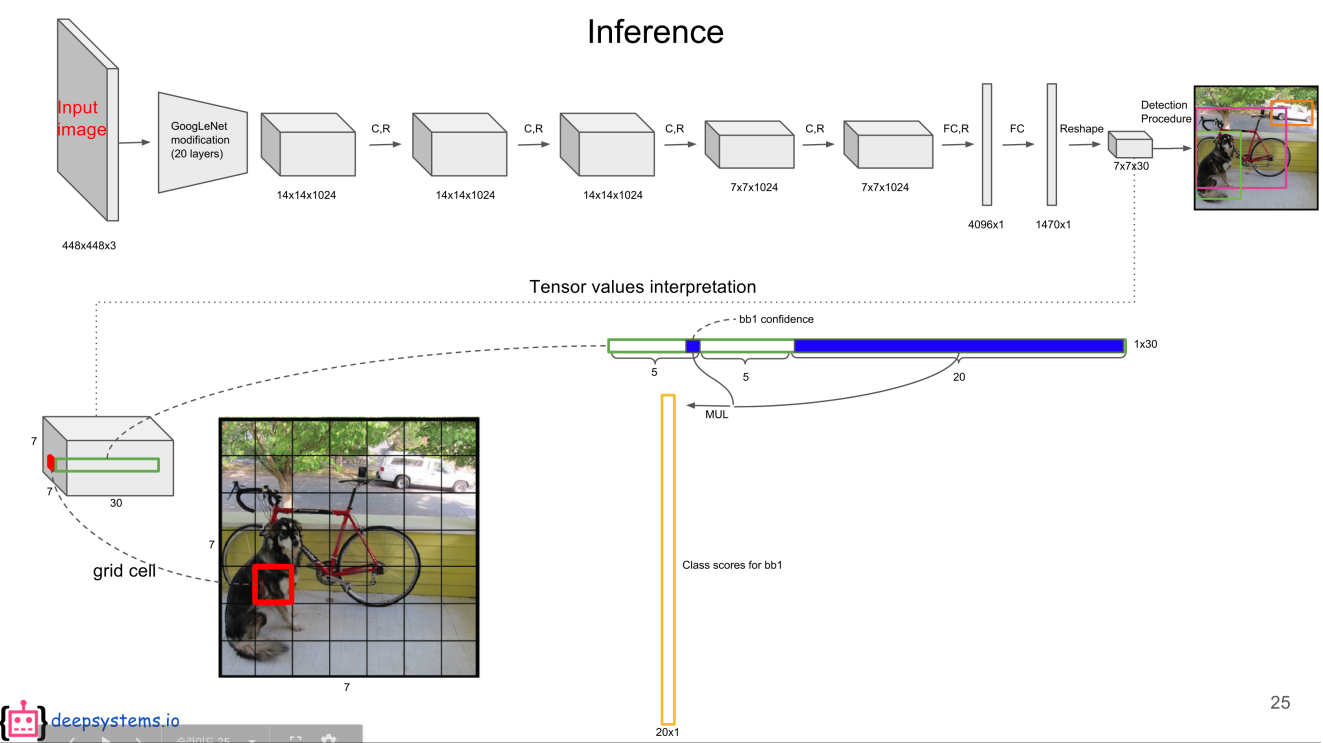
\includegraphics[width=0.6\textwidth]{images/2a-sign/yolo1_inference.png}
\end{figure}
Sau đó chúng ta cần biến đổi một chút để có được class score cho mỗi bounding box như đã trình bày ở phần trên. Chúng ta có tổng cộng 98 predicted bounding boxes. Quá trình NMS có thể được tóm tắt như hình dưới đây:
\newpage
\begin{figure}[h]
        \centering
        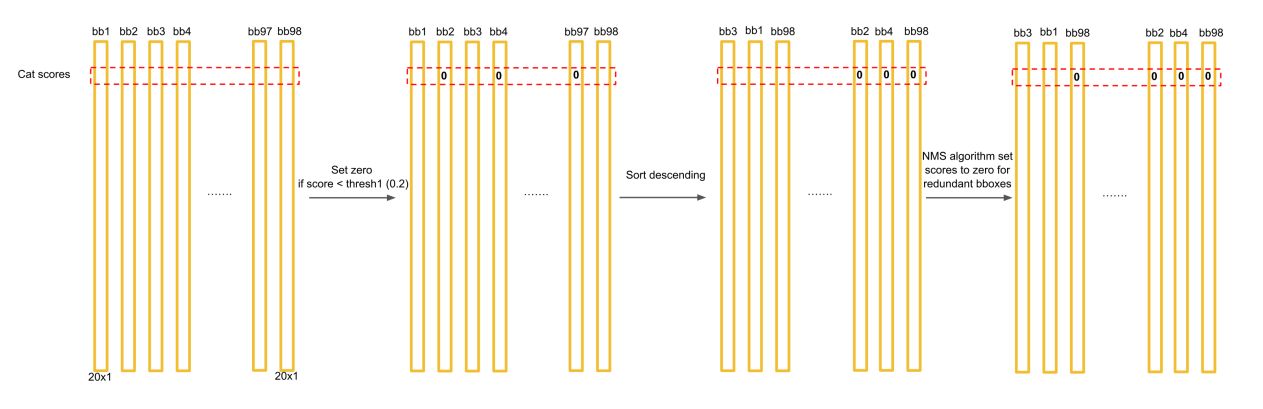
\includegraphics[width=0.8\textwidth]{images/2a-sign/yolo1_nms.png}
\end{figure}

Để đơn giản gọi $Pr(class_i) \cdot IOU_{pred}^{truth}$ là class confidence - kết quả sau khi thực hiện phép nhân. Xét cho tất cả bounding boxes:
\begin{itemize}
    \item Đối với $c_1$ class đầu tiên, nếu class confidence $c_1$ 
 của box nào nhỏ hơn threshold score thì set class confidence của box đó = 0
 \item Sắp xếp boxes theo chiều giảm của class confidence $c_1$
 \item Áp dụng NMS bắt đầu từ box bên trái có class confidence 
 $c_1$ lớn nhất, các box phía bên phải có IOU so với box đầu lớn hơn IOU threshold thì set class confidence của box đó = 0.
 \item Làm xong với box bên trái có class confidence $c_1$
 max rồi sẽ làm tiếp đến box còn lại (có class confidence $c_1$
 còn khác 0)
\item Cứ làm như vậy đến khi bên tay phải không còn box nào có class confidence $c_1$ khác 0. Như vậy xong cho một class. Lúc này class confidence của class đó trong các boxes được chọn sẽ lớn hơn 0, và bằng 0 trong các boxes không được chọn.
\item Lặp lại các bước trên lần lượt cho các class còn lại.
\end{itemize}
Sau khi thực hiện xong các bước trên sẽ đến bước vẽ các bounding box. Nên nhớ sau khi xử lý trong một bounding box có thể có nhiều class confidences khác 0. Đối với mỗi bounding box sẽ chọn ra class có confidence lớn nhất. Giá trị của class confidence này phải lớn hơn 0. Khi đó bounding box là hợp lệ có chứa thông tin class, class confidence và các thông số hình học.
\begin{figure}[htbp]
        \centering
        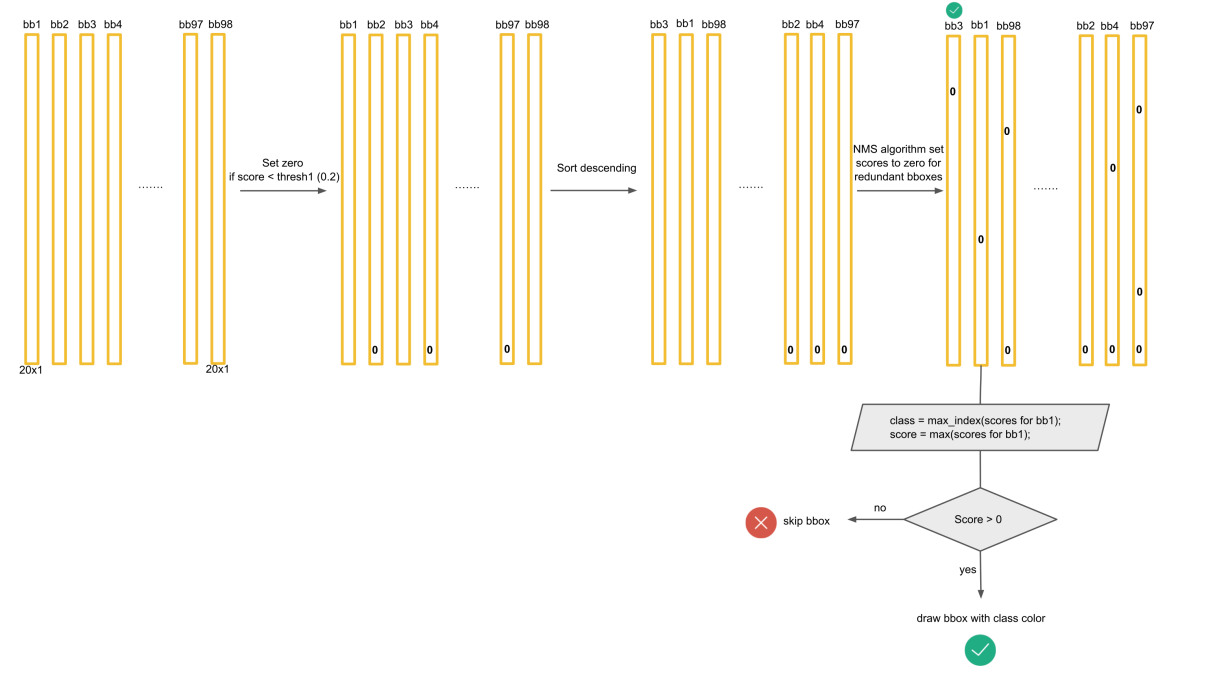
\includegraphics[width=0.8\textwidth]{images/2a-sign/yolo1_nms2.png}
\end{figure}

\subsubsection{YOLOv3}
YOLOv3 có kiến trúc khá giống YOLOv2. Tác giả đã thêm các cải tiến mới trong các nghiên cứu object detection thời điểm đó vào YOLOv2 để tạo ra YOLOv3. Base network mới được dùng, lớn hơn Darknet-19 nhưng vẫn đảm bảo được tốc độ inference.
\myparagraph{Dự đoán bounding box}
Trong dự đoán của mỗi box sẽ có các giá trị $t_x, t_y, t_w, t_h$ và objectness prediction - những giá trị này được sử dụng để tính loss. Nếu grid cell offset so với góc trên bên trái của ảnh $(c_x, c_y)$ và anchor box có width và height $p_w, p_h$ thì predictions (được tính toán lại, không phải output của model) sẽ là
\begin{equation*}
    \begin{aligned}
b_x &= \sigma(t_x) + c_x\\
b_y &= \sigma(t_y) + c_y\\
b_w &= p_w e^{t_w}\\
b_h &= p_h e^{t_h}\\
\end{aligned}
\end{equation*}
\begin{figure}[htp]
    \centering
    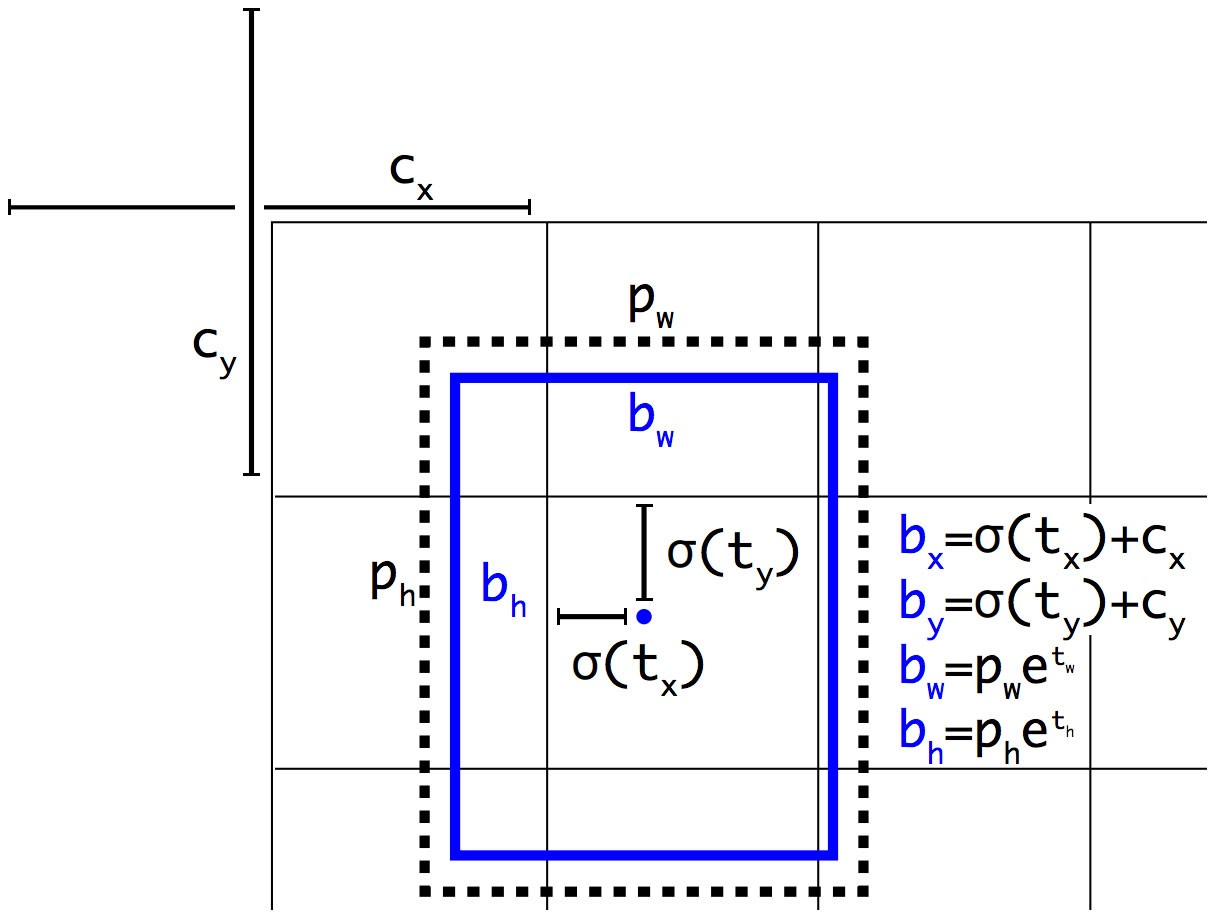
\includegraphics[width=0.4\textwidth]{images/2a-sign/yolov3.jpeg}
    \caption{Bounding box location prediction}
\end{figure}

$(c_x, c_y)$ - tọa độ góc trên bên trái của grid cell chứa anchor box tương ứng. Tọa độ này được xác định sau khi đã chia grid cell, ví dụ như hình bên trên $c_x = 1, c_y = 1$. $p_w, p_h$ cũng vậy,cũng được normalize theo width và height sau khi đã chia grid cell.\\
\newline
YOLOv3 dự đoán objectness score cho mỗi bounding box bằng logistic regression. Nếu bounding box prior (anchor) overlap với ground-truth box lớn hơn so với các anchor boxes khác thì objectness score bằng 1. Nếu anchor box không có IoU lớn nhất nhưng overlap với ground-truth box và IoU lớn hơn threshold 0.5 thì chúng ta bỏ qua dự đoán đó - không tính loss. Mỗi ground-truth box chỉ liên quan đến một anchor box. Nếu anchor box không được gán cho ground-truth box nào thì khi tính loss cho nó sẽ bỏ qua classification loss, localization loss và chỉ tính confidence loss cho object - liên quan đến việc có object hay không.

\myparagraph{Dự đoán các lớp}
Mỗi box dự đoán các classes mà box đó có thể chứa bằng multilabel classification. Chúng ta không sử dụng softmax và thay vào đó sử dụng các logistic classifiers độc lập với nhau. Trong suốt quá trình training thì sử dụng binary cross-entropy loss cho class predictions. Thông thường chỉ sử dụng softmax khi mỗi box có duy nhất một class, tuy nhiên với nhiều dataset các objects có thể rất gần nhau và việc sử dụng này không hiệu quả.

\myparagraph{Trích xuất đặc trưng}
YOLOv3 sử dụng mạng neural network mới để trích xuất đặc trưng Darknet-53. Darknet-53 vẫn dựa trên sự thành công của 3x3, 1x1 Conv layers giống như kiến trúc Darknet-19 cũ, tuy nhiên ở đây sử dụng thêm residual blocks. Model mới có 53 Conv layers nên gọi là DarkNet-53.
\begin{figure}[htp]
    \centering
    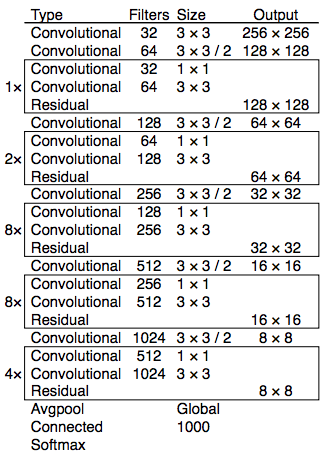
\includegraphics[width=0.4\textwidth]{images/2a-sign/yolov3_archi.png}
    \caption{Kiến trúc Darknet-53}
\end{figure}

\noindent Darknet-53 mạnh mẽ hơn so với Darknet-19. Darknet-53 tốt hơn so với ResNet-101 và nhanh hơn 1.5 lần. Darknet-53 có performnace tương đương ResNet-152 nhưng nhanh hơn 2 lần.\\

\noindent Darknet-53 có BFLOP/s (billion floating point operations per second) lớn. Điều này có nghĩa rằng kiến trúc của Darknet-53 sử dụng tốt GPU, giúp nó có tốc độ nhanh hơn.
\myparagraph{Multi-scale prediction}
YOLOv3 đưa ra dự đoán cho 3 scales khác nhau. YOLOv3 trích xuất features từ những scales này bằng cách sử dụng khái niệm tương tự Feature Pyramid Network. Từ base feature extractor sẽ thêm một số Conv layers.\\
Ở mỗi scale sẽ dự đoán 3 boxes cho mỗi vị trí (grid cell), do đó output tensor cho mỗi scale là N x N x [3 x (4 + 1 + 80)] với:
\begin{itemize}
    \item 4 bounding box offsets
    \item 1 objectness prediction
    \item 80 class predictions
\end{itemize}
Cụ thể việc dự đoán cho 3 scales khác nhau là:
\begin{itemize}
    \item Ở feature map cuối cùng
    \item Feature map ở trước đó 2 layers, feature map được được upsample 2x. YOLOv3 lấy feature map có resolution lớn hơn (ở trước nữa trong mạng NN) và kết hợp với upsampled feature thông qua concatenation. Sau đó áp dụng một số Conv layers và dự đoán output cuối cùng.
    \item Thực hiện thiết kế như scale thứ 2 cho scale thứ 3.
\end{itemize}

\begin{figure}[htp]
    \centering
    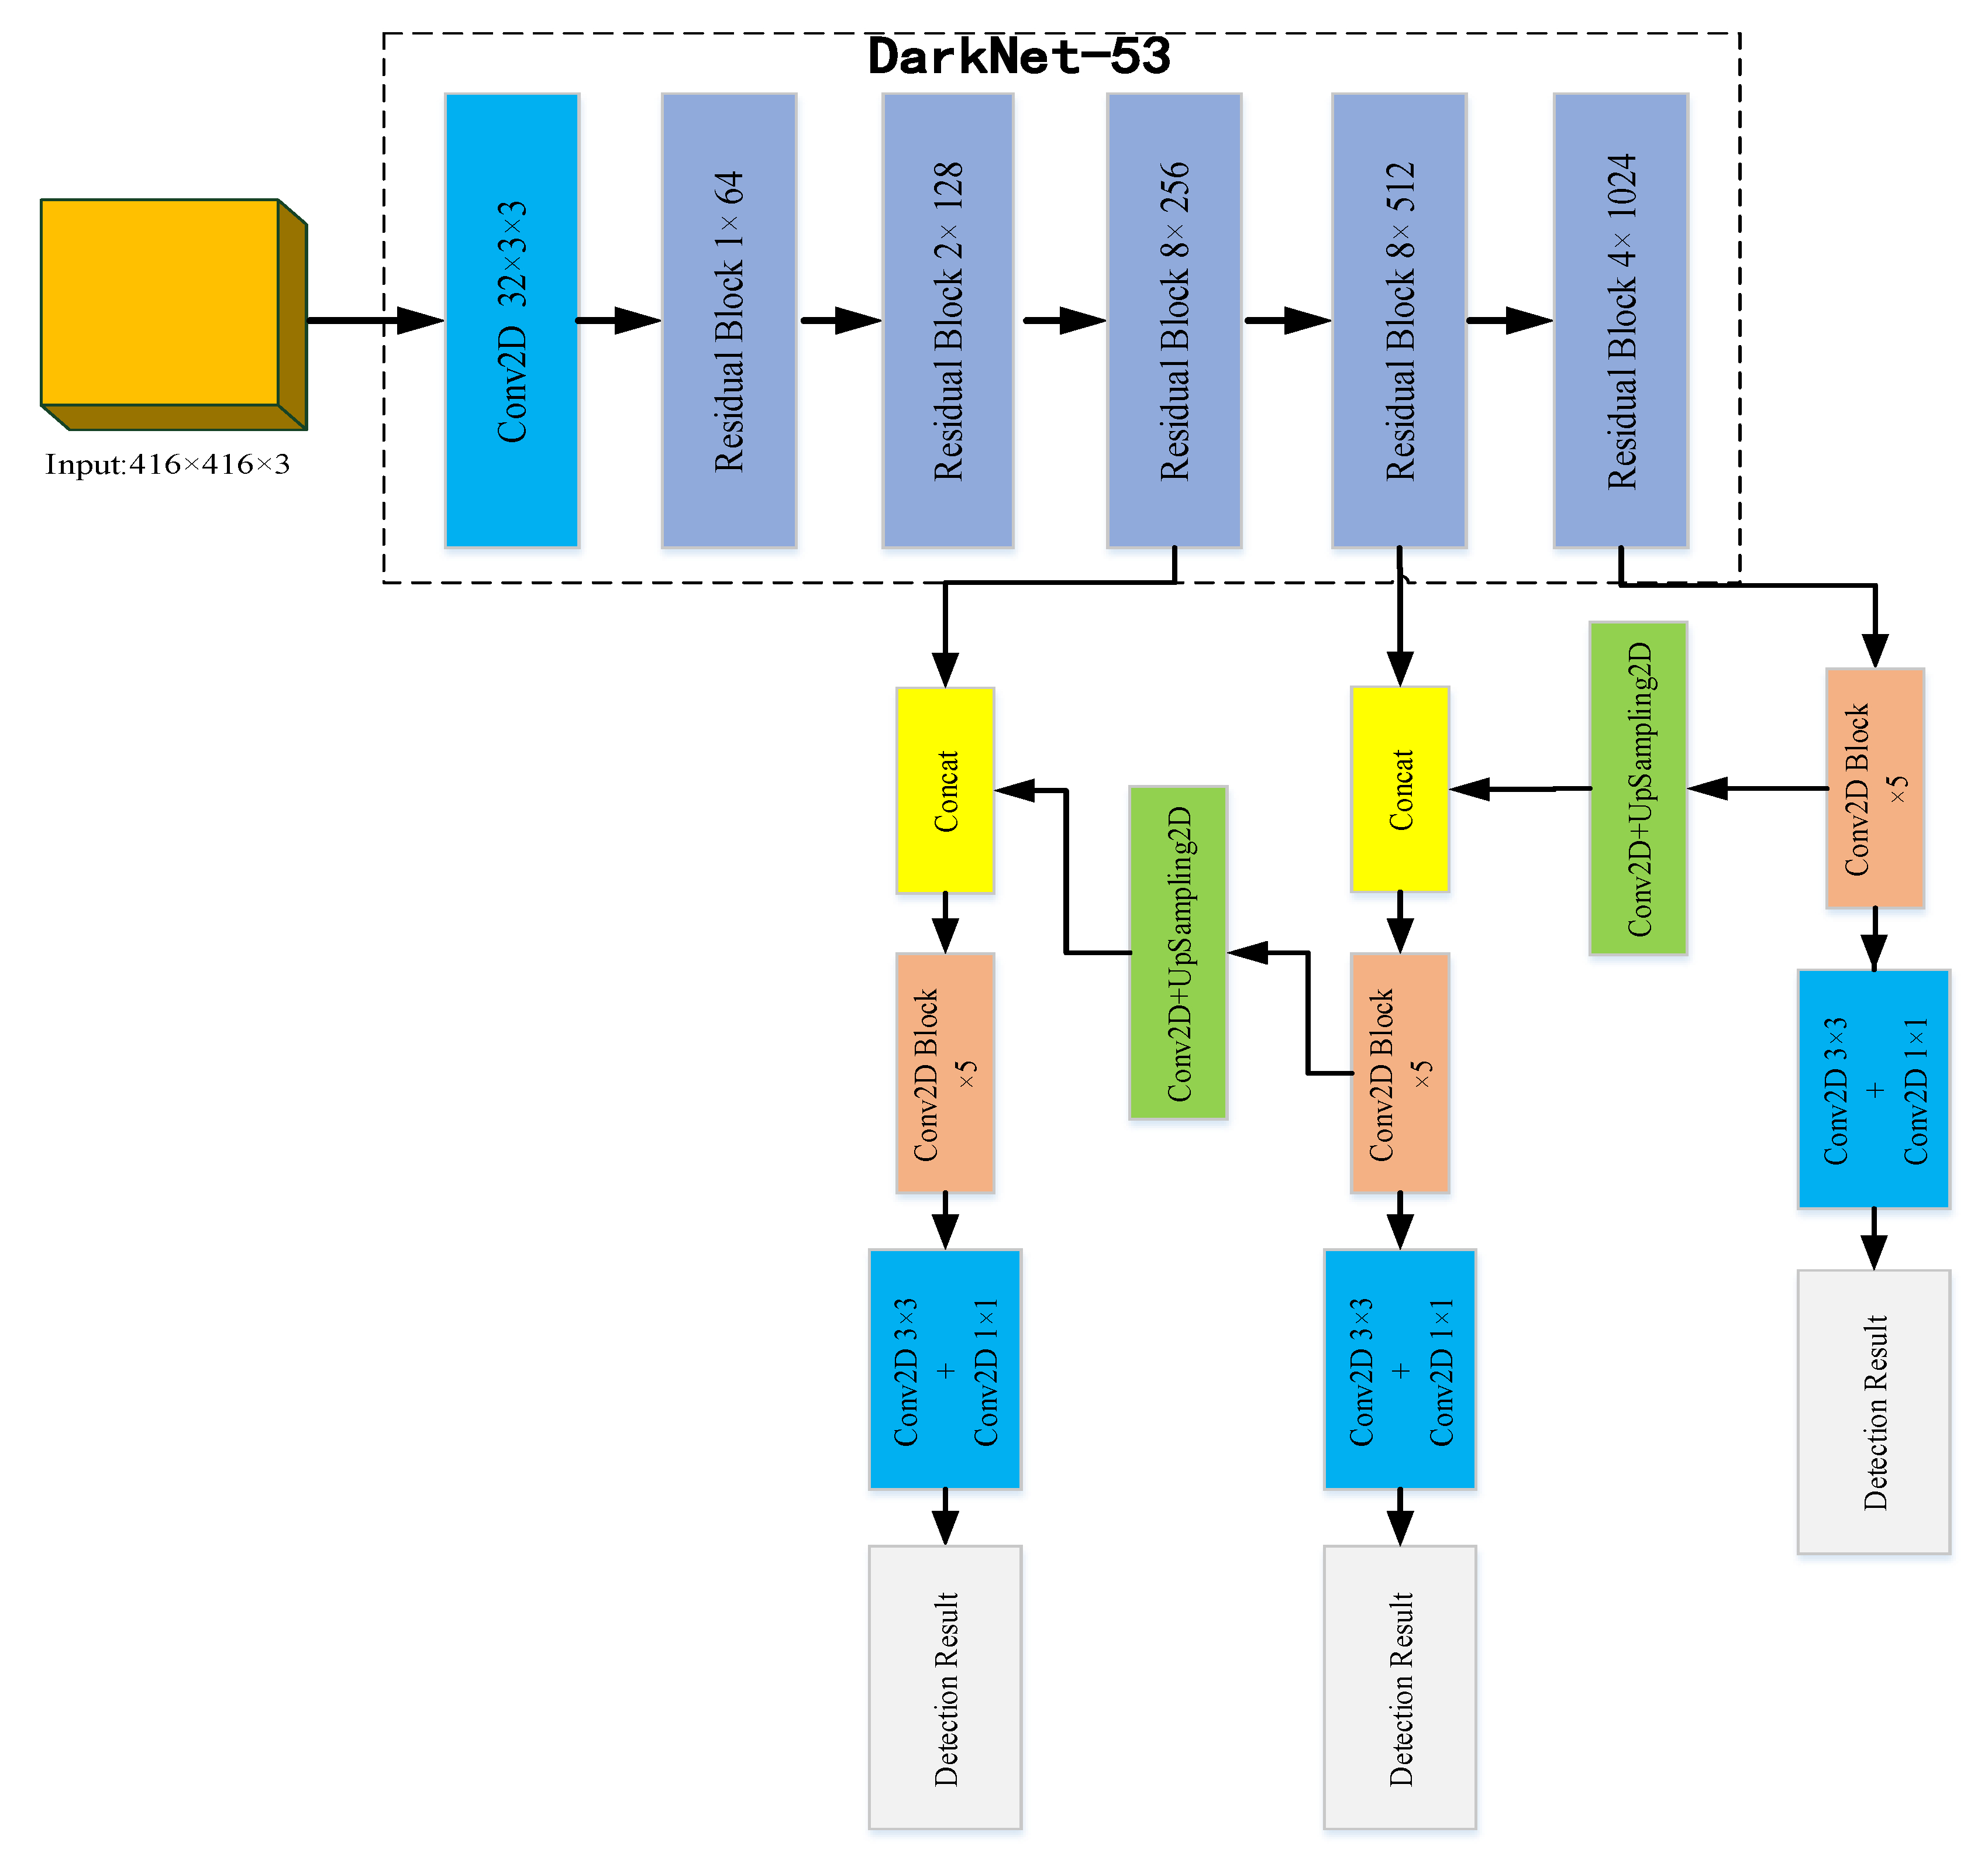
\includegraphics[width=0.6\textwidth]{images/2a-sign/YOLOv3-arch.jpg}
    \caption{Kiến trúc YOLOv3}
\end{figure}

\noindent Chính việc dự đoán với các scales khác nhau mà YOLOv3 đã cải thiện khi dự đoán các object nhỏ.

\noindent YOLOv3 vẫn sử dụng K-Means để chọn ra trước 9 prior boxes (anchor boxes). Đối với COCO dataset, width và height của mỗi anchor box là (10×13), (16×30), (33×23), (30×61), (62×45), (59× 119), (116 × 90), (156 × 198), (373 × 326).





